\section{Flussprobleme}

\begin{definition}
    \index{Netzwerk}
    \index{Quelle}
    \index{Ziel}

    Ein \emph{Netzwerk} besteht aus $3$ Komponenten:
    \begin{enumerate}
        \item einem endlichen gerichteten Graph $G = (V, E)$ ohne Schleifen
            (Kanten von $v_i$ zum selben Knoten $v_i$) und ohne parallele Kanten,
        \item einer Funktion $c$, $c:E \rightarrow \mathbb{R}^{+}$, die jeder
            Kante $e \in E$ ihre Kapazität zuordnet,
        \item $2$ ausgezeichneten Knoten $s$ und $t$, genannt \emph{Quelle} und
            \emph{Ziel}. Diese Knoten müssen nicht im Graphentheoretischen Sinne
            Quelle und Senke sein.
    \end{enumerate}

    Soll ein Graph mit parallelen Kanten in ein Netzwerk überführt werden,
    ersetzt man alle parallelen Kanten durch jeweils nur eine Kante. Die
    Kapazität dieser neuen Kante ist gleich der Summe der Kapazitäten der
    Kanten, die sie ersetzt:
    %TODO bild
    
    Schleifen $e = (v, v)$ ergeben im Kontext von Flussproblemen keinen Sinn.
    Falls sie trotzdem in einem Netzwerk dargestellt werden sollen, kann man
    sie durch Kanten $e' = (v, v')$ und $e'' = (v', v)$ zu einem neuen Knoten
    $v'$ darstellen.
    %TODO bild
\end{definition}


\begin{definition}
    \index{Flussfunktion}
    \index{Flusserhaltungsgesetz}
    \index{Fluss!totaler Fluss}

    Eine \emph{Flussfunktion} für ein Netzwerk $(G, c, s, t)$ ist eine Funktion
    $f:E \rightarrow \mathbb{R}$, für die gilt:
    \begin{enumerate}
        \item $0 \leq f(e) \leq c(e)$
        \item sei $\alpha(v) = \{ e: e \text{ führt zu } v \}$, $\beta(v) = \{
            e: e \text{ führt aus } v \}$, $v \in V$ Knoten, dann gilt $\forall v$
            mit $v \neq s$ und $v \neq t$ das \emph{Flusserhaltungsgesetz}:
            $$ \sum_{e \in \alpha(v)} f(e) = \sum_{e \in \beta(v)} f(e) $$
            %TODO bild
    \end{enumerate}

    \noindent
    Sei $f$ eine Flussfunktion, dann heißt $$F = \sum_{e \in \alpha(t)} f(e)
    - \sum_{e \in \beta(t)} f(e)$$ der \emph{totale Fluss} von $f$. Der totale
    Fluss bezieht sich stets auf das -- frei wählbare -- Ziel des Netzwerks
    $t$.
\end{definition}


\begin{bemerkung}
    Eine typische Aufgabe ist es, zu einem Netzwerk eine Flussfunktion $f$ zu
    suchen, so dass ihr totaler Fluss $F$ maximal ist.
\end{bemerkung}


\begin{definition}
    \index{Schnitt}
    \index{Schnitt!Kapazität}

    Sei $S \subseteq V$ mit $s \in S$, $\overline{S} = V \setminus S, t \in
    \overline{S}$.

    $E_{S\overline{S}} = \{ e: \text{ Anfangspunkt von $e \in S$}, \text{
    Endpunkt von $e \in \overline{S}$}\}$

    $E_{\overline{S}S} = \{ e: \text{ Anfangspunkt von $e \in \overline{S}$},
    \text{ Endpunkt von $e \in S$}\}$

    %TODO bild
    
    Der durch $S$ definierte \emph{Schnitt} ist die Menge $E_{S\overline{S}}
    \cup E_{\overline{S}S}$. Die Kapazität des durch $S$ definierten Schnitts
    ist $$c(S) = \sum_{e \in E_{S\overline{S}}} c(e) \qquad \text{(Beachte:
    dies ist die Kapazität in Richtung $\overline{S}$, $t \in \overline{S}$)}$$
\end{definition}


\begin{lemma}
    \label{totalerfluss}
    Sei $N = (G, c, s, t)$ ein Netzwerk, und $f$ eine Flussfunktion für $N$.
    Dann gilt $\forall S \subseteq V$ mit $s \in S$ und $t \notin S$: $$
    F = \sum_{e \in E_{S\overline{S}}} f(e) - \sum_{e \in E_{\overline{S}S}}
    f(e)$$
    Egal welches $S$ man wählt, der totale Fluss (gebunden an $t$) lässt sich
    damit berechnen.
\end{lemma}


\begin{beweis}
    \setcounter{equation}{0}
    \begin{align}
        0 &= \sum_{e \in \alpha(v)} f(e) - \sum_{e \in \beta(v)} f(e) \qquad
          \forall v, v \neq s, v \neq t, \text{ weil $f$ Flussfunktion} \\
        F &= \sum_{e \in \alpha(t)} f(e) - \sum_{e \in \beta(t)} f(e) \qquad
        \text{ Definition von $F$}
    \end{align}

    Addiere Gleichung $(1)$ für alle $v \in \overline{S} \setminus \{t\}$ zu
    Gleichung $(2)$. Auf der linken Seite der Ergebnisgleichung steht $F$. Im
    folgenden bestimmen wir die rechte Seite. Betrachte alle Kanten in $E$: sei
    $e \in E$ mit $x \stackrel{e}{\rightarrow} y$.
    \begin{itemize}
        \item Fall 1: $x, y \in S$: dann kommt $f(e)$ in der Summation nicht
            vor (es wird nur über $v \in \overline{S} \setminus \{t\}$ summiert).
        \item Fall 2: $x, y \in \overline{S}: e \in \alpha(x), e \in \beta(x)$,
            also heben sich die Werte von $f(e)$ bei der Summation gegenseitig auf.
        \item Fall 3: $x \in S, y \in \overline{S}: f(e)$ ist positiv für $y$,
            für $x$ kommt es nicht in der Summation vor, $e \in E_{S\overline{S}}$.
        \item Fall 4: $x \in \overline{S}, y \in S: f(e)$ ist negativ für $x$,
            kommt für $y$ nicht in der Summation vor, $e \in E_{\overline{S}S}$.
    \end{itemize}

    Bei der Summation über die rechte Seite ergibt sich: $$ \sum_{e \in
    E_{S\overline{S}}} f(e) - \sum_{e \in E_{\overline{S}S}} f(e) \qquad
    \text{(Fall 3 - Fall 4)}$$
\end{beweis}


\begin{beispiel}
    Schreibweise: $\nicefrac{c}{f} \qquad \nicefrac{\text{Kapazität}}{\text{Fluss}}$
    %TODO bild
\end{beispiel}


\begin{lemma}
    \label{flusskleinerkap}
    Für jede Flussfunktion $f$ mit totalem Fluss $F$ und für jedes $S \subseteq
    V$ mit $s \in S, t \notin S$ gilt: $F \leq c(S)$.
\end{lemma}


\begin{beweis}
    Aus Lemma \ref{totalerfluss} folgt:
    $$ F_{3.1} = \sum_{e \in E_{S\overline{S}}} f(e) - \sum_{e \in
    E_{\overline{S}S}} \leq \sum_{e \in E_{S\overline{S}}} f(e) \leq \sum_{e
    \in E_{S\overline{S}}} c(e) \stackrel{\text{Def}}{=} c(S)$$
\end{beweis}


\begin{korollar}
    \index{Max Flow Min Cut}
    
    \emph{Max Flow Min Cut-Theorem}: Sei $f$ eine Flussfunktion und $S
    \subseteq V, s \in S, t \notin S$. Wenn $F = c(S)$, dann ist $f$ eine
    Flussfunktion mit maximalem totalen Fluss und die Kapazität des durch $S$
    definierten Schnittes ist minimal.
\end{korollar}


\begin{beweis}
    Sei für ein $f$ und ein $S$ der totale Fluss $F = c(S)$. Sei $f'$ eine
    andere Flussfunktion mit totalem Fluss $F'$. Aus Lemma
    \ref{flusskleinerkap} folgt: $F' \leq c(S) = F$, also ist $F$ maximal.

    Sei $S' \subseteq V$ mit $s \in S', t \notin S'$. Dann gilt:
    $\underset{=c(S)}{F} \leq c(S)$, also ist $c(S)$ minimal.
\end{beweis}


\begin{definition}
    \index{Anreicherungspfad}
    \index{Augmenting Path}

    Gegeben sei ein Netzwerk $(G, c, s, t)$ und eine Flussfunktion $f$ für
    dieses Netzwerk. Ein \emph{Anreicherungspfad} (Augmenting Path) ist ein
    einfacher Pfad oder Weg von $s$ nach $t$, der nicht notwendigerweise
    gerichtet ist, und für den gilt: Sei $e$ eine Kante auf diesem Weg: 

    \begin{center}
        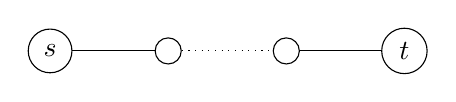
\begin{tikzpicture}
            \node (s) at (0, 0) [draw, shape=circle] {$s$};
            \node (v1) at (1.5, 0) [draw, shape=circle] {};
            \node (v2) at (3, 0) [draw, shape=circle] {};
            \node (t) at (4.5, 0) [draw, shape=circle] {$t$};

            \draw (s) -- (v1);
            \draw (v2) -- (t);
            \draw[dotted] (v1) -- (v2);
        \end{tikzpicture}
    \end{center}

    \begin{itemize}
        \item Fall 1: $e$ ist eine \emph{Vorwärtskante}, d.h. \\
            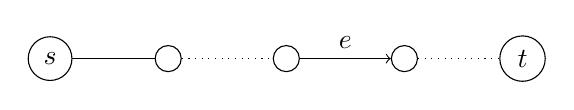
\begin{tikzpicture}
                \node (s) at (0, 0) [draw, shape=circle] {$s$};
                \node (v1) at (1.5, 0) [draw, shape=circle] {};
                \node (v2) at (3, 0) [draw, shape=circle] {};
                \node (v3) at (4.5, 0) [draw, shape=circle] {};
                \node (t) at (6, 0) [draw, shape=circle] {$t$};

                \draw (s) -- (v1);
                \draw[->] (v2) -- (v3);
                \draw[dotted] (v3) -- (t);
                \draw[dotted] (v1) -- (v2);

                \node (e) at (3.75, 0.2) {$e$}; 
            \end{tikzpicture} \\
            dann muss $f(e) < c(e)$ sein.
        \item Fall 2: $e$ ist eine \emph{Rückwärtskante}, d.h. \\
            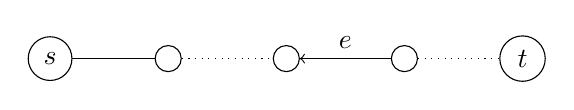
\begin{tikzpicture}
                \node (s) at (0, 0) [draw, shape=circle] {$s$};
                \node (v1) at (1.5, 0) [draw, shape=circle] {};
                \node (v2) at (3, 0) [draw, shape=circle] {};
                \node (v3) at (4.5, 0) [draw, shape=circle] {};
                \node (t) at (6, 0) [draw, shape=circle] {$t$};

                \draw (s) -- (v1);
                \draw[<-] (v2) -- (v3);
                \draw[dotted] (v3) -- (t);
                \draw[dotted] (v1) -- (v2);

                \node (e) at (3.75, 0.2) {$e$};
            \end{tikzpicture} \\
            dann muss $f(e) > 0$ sein.
    \end{itemize}
\end{definition}


\begin{beispiel}
    %TODO bild und so
\end{beispiel}


\begin{definition}
    \index{Vorwärtsmarkierung}
    \index{Rückwärtsmarkierung}

    Eine \emph{Vorwärtsmarkierung} des Knoten $v$ durch die Kante 
    \begin{tikzpicture}[baseline]
        \node (u) at (0, 0) {$u$};
        \node (v) at (1.5, 0) {$v$};
        \draw[->] (u) -- (v);
        \node (e) at (0.75, 0.2) {$e$};
    \end{tikzpicture}
    ist anwendbar, wenn \begin{enumerate}
        \item $u$ markiert ist und $v$ nicht, und
        \item $f(e) > 0$.
    \end{enumerate}
    $v$ erhält dann die Markierung ``$e$'' (Name der Kante). 
    
    Eine \emph{Rückwärtsmarkierung} des Knoten $v$ durch die Kante 
    \begin{tikzpicture}[baseline]
        \node (u) at (0, 0) {$u$};
        \node (v) at (1.5, 0) {$v$};
        \draw[<-] (u) -- (v);
        \node (e) at (0.75, 0.2) {$e$};
    \end{tikzpicture}
    ist anwendbar, wenn \begin{enumerate}
        \item $u$ markiert ist und $v$ nicht, und
        \item $f(e) > 0$.
    \end{enumerate}
    $v$ erhält dann die Markierung ``$e$''. 

    Im 1. Fall, also bei Vorwärtsmarkierung, wird $\Delta(e) = c(e) - f(e)$. Im 2. Fall wird $\Delta(e) = f(e)$. In beiden Fällen ist $\Delta(e) > 0$.
\end{definition}


\begin{definition}
    \index{Ford-Fulkerson-Algorithmus}

    \emph{Algorithmus von Ford und Fulkerson zur Bestimmung einer Flussfunktion mit maximalem totalen Fluss}. Gegeben sei ein Netzwerk $(G, c, s, t)$ und eine Flussfunktion $f$ für dieses Netzwerk. Der folgende Algorithmus verändert $f$ mit dem Ziel, den totalen Fluss zu maximieren.

    \begin{enumerate}
        \item Setze $f(e) := 0 \qquad \forall e \in E$
        \item Kennzeichne $s$ als ``markiert'' und alle anderen Knoten als ``unmarkiert''
        \item Suche einen Knoten $v$, der vorwärts oder rückwärts markiert werden kann. Gibt es keinen solchen Knoten, dann halte an. Das damit gefundene $f$ hat maximalen totalen Fluss. Gibt es einen solchen Knoten $v$, dann markiere $v$ mit der Kante $e$, die zur Markierung geführt hat. Ist $v = t$, dann gehe zu Schritt 4, ansonsten zu Schritt 3.
    \end{enumerate}
\end{definition}
